\section{RISC-V}
%file://icnas2.cc.ic.ac.uk/cmg1418/downloads/riscv-spec-20191213.pdf
%https://www2.eecs.berkeley.edu/Pubs/TechRpts/2016/EECS-2016-161.pdf
%https://www.cnx-software.com/2019/08/27/risc-v-bases-and-extensions-explained/
%https://en.wikichip.org/wiki/risc-v/standard_extensions

RISC-V\cite{RVISAManualVol1} is an open standard instruction set architecture which aims to support computer architecture research, education and provides a free architecture for those in industry to implement.
Since RISC-V is an open standard that is designed to be extensible, there are many tools chains that support development of software, custom instructions and their associated hardware.
The open nature of RISC-V also means there is open work being done on soft RISC-V cores. This means I will be able to use and modify a preexisting core to function will my custom hardware and instruction.

\subsection{Standard Instruction Set Extensions}


RISC-V is also designed to be highly extensible and customisable. It provides a base integer instruction sets in 32, 64 and 128-bit forms which can be extended using one of the many standard extensions that have been developed. As well as this there is extensive support in the instruction space for the addition of custom instructions with base length or with extended length.

These are ratified extensions meaning they are officially supported by the RISC-V specification. These extensions can be removed from ratification and modified but for the purposes of this project we will assume that the all the standard extensions being used will remain ratified.

A general purpose ISA's have been defined by the RISC-V specification Chapter 24. These being RV32G and RV64G, with G standing for "general". These are a combination of the base 32-bit and 64-bit integer instruction sets and the following standard extensions \cite{RVISAManualVol1}:
\begin{itemize}
    \item I - Base instruction set for integer operations
    \item M - Integer multiplication and division
    \item F - Single precision floating-point operations
    \item A - Atomic operations
    \item D - Double precision floating-point operations
    \item Zicsr - Control and status register instructions
    \item Zifencei - Instruction-fetch and fence instructions
\end{itemize}

These are likely the best supported extensions and will likely be supported as a group, therefore I will be using only these. The vector extension "V", may prove useful for performance enhancement in the future however, software optimisation is not th efocus of this project and so the use of vector instructions is out of scope. As well as this the "V" instruction set is still in its draft phase and so any work done using it may be wasted.

For the purposes of this project a bare metal execution environment will be used.

There are several of the "G" extensions, that will prove useful, mainly F and M since floating point operations are critical in graphics applications, however there are cases where fixed point arithmetic is used. The differences between fixed point and floating point precision will be explored later in the project.
\todo{Make experiments to explore difference between fixed and floating point rendering algorithms}

RISC-V has little-endian instructions (normal endianness). The prefix indicates the major opcodes which are used by certain instruction types. 
\subsection{Custom Instruction Set Extensions}

\begin{figure}[ht]
    \centering
    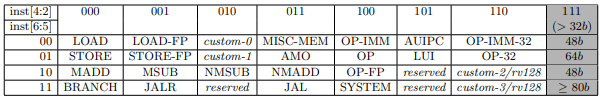
\includegraphics{lit_review/images/RV32G_64G_InstructionSetTable.png}
    \caption{Instruction Set Listing for RV32G and RV64G, inst[1:0] = 11}
    \label{fig:RV32G_64G_InstructionSetTable}
\end{figure}
As shown by \ref{fig:RV32G_64G_InstructionSetTable}, there are 4 major opcodes reserved for custom instructions. Ideally, I would like to allow my instruction to be used by RV128 in the future, therefore I will avoid using the custom-2 and custom-3 opcodes. 
I will likely use the custom-0 or custom-1 opcodes for my instruction. The format of the rest of the instruction is entirely up to me. To implement what I want I just have to add compiler support and to alter a decode unit from a risc-v core to make it able to decode my instruction.

Brownfield and Greenfield extensions. 
\subsection{RISC-V Open-Source CPU Cores}
There are numerous open-source RISC-V cores that support RV32I and M \cite{nolting22}\cite{ibex}\cite{wyvernsemiriscV}. The cited cores are all in-order cores, which although making them lower performance, than an out of order (OOO) core, makes them much simpler to modify for the purposes of my project. 

One major issue I ran into, however, is that the only open-source cores that I could find that would support all of the \textit{G} extension, are the Berkeley BOOM \cite{zhaosonicboom} core and the Rocket Chip \cite{Asanovic-EECS-2016-17}. These are out of order and in order cores respectively. However, BOOM only support RV64G so if I choose to use this core I will need to move to using a 64 bit ISA. This will not add too much complexity.

The problem with this is that they are both written in Chisel, a domain-specific language (DSL) in Scala. In both cases the Chisel design compiles to autogenerated Verilog which is likely to be completely unreadable. 

\begin{shaded}
This presents a question of how I should go about modifying the cores to add my design. I can:
\begin{enumerate}
    \item Write my design in Chisel and modify the Chisel
    \item Write my design in SystemVerilog and either:
    \subitem Modify the Verilog generated directly to add my design
    \subitem Modify the Chisel of the CPU core and somehow integrate my SystemVerilog design with the Chisel.
    \item Continue looking for a core that is hand written in Verilog or SystemVerilog
\end{enumerate}
\end{shaded}
\todo{answer the above question}

Both the BOOM and Rocket Cores are supported by the Chipyard\cite{chipyard} framework for the Agile development of RISC-V SoC's. This framework could greatly help in speeding up the design process of my core hardware if it allows for the addition of custom hardware. Additional research will need to be done to see if it allows this and if it allows the addition of Verilog code or only Chisel code.

\section{Tools}
RISC-V Tools repo
GNU RISC-V Toolchain
Bare metal executiono environment
need a RV32G cross compiler for C++
need an architectural simulator
hardware design tools, quartus prime for FPGA implementation
yosys - open source RTL simulation software
verilator - open source verilog synthesiser

I will use SystemVerilog, provides some nice high level functionality, packages, structs. Also provides nice verification features which will be a key part of my project when design starts.